\documentclass[conference]{IEEEtran}
\IEEEoverridecommandlockouts % show footnote comments

\usepackage{cite}
\usepackage{graphicx}
\usepackage{textcomp}
\usepackage{xcolor}
\usepackage{balance}
\usepackage{booktabs}
\usepackage{pifont}
\usepackage{pgfplots}
\usepackage{pgfplotstable}
\pgfplotsset{compat=newest}
\usepackage{comment}
\usepackage{multirow}
\usepackage[bookmarks=false]{hyperref}
\hypersetup{
    pdftitle = {ePMapping: A Staged Rewriting Framework for Post-Mapping Area Optimization},
    colorlinks = true,
    citecolor  = blue,
    linkcolor  = blue,
    urlcolor   = blue,
}
\usepackage{resizegather}
\usepackage[subrefformat=parens,farskip=0pt,justification=centering]{subfig}
\captionsetup[subfigure]{subrefformat=simple,labelformat=simple,listofformat=subsimple}
\renewcommand\thesubfigure{(\alph{subfigure})}
\usepackage[labelsep=period,font=small]{caption}
\usepackage{url}
\usepackage{threeparttable}
\usepackage{physunits}
\usepackage[round-pad=false,round-mode=places,round-precision=2,group-separator={,},output-decimal-marker={.},per-mode=symbol]{siunitx}

\usepackage{amsthm}
\newtheorem{lemma}{Lemma}
\newtheorem{theorem}{Theorem}
\newtheorem{definition}{Definition}
 
\makeatletter
\newif\if@restonecol
\makeatother
\let\algorithm\relax
\let\endalgorithm\relax
\usepackage[linesnumbered,ruled,vlined]{algorithm2e}
\usepackage{algpseudocode}
\usepackage{amsmath,amsfonts}
\renewcommand{\algorithmicrequire}{\textbf{Input:}} % Use Input in the format of Algorithm
\renewcommand{\algorithmicensure}{\textbf{Output:}} % Use Output in the format of Algorithm
\SetKwRepeat{Do}{do}{while}
\SetAlgoInsideSkip{small}
%\SetAlgoHangIndent{0pt}

\usepackage{amsthm}
\usepackage{cleveref}
\Crefformat{figure}{Fig.~#2#1#3}                           % "Fig.", instead of "Figure"
\Crefname{subfigure}{Fig.}{Figs.}
\Crefname{figure}{Fig.}{Figs.}
\Crefformat{table}{TABLE~#2#1#3}                           % "TABLE", instead of "Table"
\Crefname{table}{TABLE}{TABLEs}

\usepackage{tikz}
\usetikzlibrary{positioning,arrows.meta}
\usepackage{enumitem}
\newcommand*\circled[1]{\tikz[baseline=(char.base)]{\node[shape=circle,fill=blue!20,draw,inner sep=1pt] (char) {#1};}}
\newcommand{\minisection}[1]{\vspace{.06in}\noindent{\textbf{#1}}.}
\newcommand{\todo}[1]{\textcolor{red}{[TODO: #1]}}
\newcommand{\revise}[1]{\DIFadd{#1}}
\newcommand{\ie}{\textit{i.e.}}
\newcommand{\eg}{\textit{e.g.}}
\newcommand{\etal}{\textit{et al.}}

\iftrue
    %\setlength{\columnsep}{20pt}                               % set space between columns
    \setlength{\textfloatsep}{6pt plus 1pt minus 1pt}          % set space between float and text
    \setlength{\floatsep}{2pt plus 1pt minus 1pt}              % set space between two floats
    \setlength{\intextsep}{2pt plus 1pt minus 1pt}             % set space between text and float
    \setlength{\abovecaptionskip}{4pt}                         % set space between figure and caption
    \setlength{\belowcaptionskip}{4pt}                         % set space between figure and caption
    % ==== reduce space around equations
    \setlength{\belowdisplayskip}{4pt} \setlength{\belowdisplayshortskip}{4pt}
    \setlength{\abovedisplayskip}{4pt} \setlength{\abovedisplayshortskip}{4pt}
\fi

\setcounter{dbltopnumber}{3}
\renewcommand{\dbltopfraction}{.95}
\renewcommand{\textfraction}{.05}
\setlength{\dblfloatsep}{6pt plus 1pt minus 1pt}
\graphicspath{{./figs/}{../}}

\usepackage[a4paper, total={184mm,239mm}]{geometry}
\def\BibTeX{{\rm B\kern-.05em{\sc i\kern-.025em b}\kern-.08em
    T\kern-.1667em\lower.7ex\hbox{E}\kern-.125emX}}
% GENERATED from paired CEC/PPA/cache audits.
% GENERATED from verified three-part campaign; do not edit numbers.
\newcommand{\MainWins}{14}
\newcommand{\MainAreaAll}{-9.12}
\newcommand{\MainDelayAll}{-6.92}
\newcommand{\OwnArea}{-7.11}
\newcommand{\OwnDelay}{-7.43}
\newcommand{\OwnAreaWins}{16}
\newcommand{\OwnOneArea}{-5.04}
\newcommand{\OwnOneDelay}{-4.90}
\newcommand{\ABCCompleted}{13}
\newcommand{\ABCTimeouts}{3}
\newcommand{\ABCFeasible}{6}
\newcommand{\ABCViolations}{7}
\newcommand{\ABCArea}{-3.58}
\newcommand{\ABCDelay}{+11.02}
\newcommand{\ABCGuardArea}{-1.59}
\newcommand{\ABCGuardDelay}{-0.15}
\newcommand{\MfsOwnArea}{-6.96}
\newcommand{\MfsOwnDelay}{-5.47}
\newcommand{\PairedOwnArea}{-7.06}
\newcommand{\PairedOwnDelay}{-6.61}
\newcommand{\ChainAreaWins}{1}
\newcommand{\OwnOtherArea}{-3.59}
\newcommand{\OwnOtherDelay}{-3.00}
\newcommand{\TimeSynShare}{22.4}
\newcommand{\TimeEggShare}{49.4}
\newcommand{\DeltaSyn}{+394.71}
\newcommand{\DeltaEgg}{+3.89}
\newcommand{\DeltaDB}{+1.62}
\newcommand{\DeltaCare}{+15.16}
\newcommand{\DeltaChain}{+334.08}
\newcommand{\DeltaShare}{+334.08}
\newcommand{\ColdMainSeconds}{3222.0}
\newcommand{\WarmMainSeconds}{1900.0}
\newcommand{\ColdMfsSeconds}{1848.2}
\newcommand{\WarmMfsSeconds}{959.4}
\newcommand{\WarmTimeEggShare}{13.9}
\newcommand{\WarmTimeSynShare}{38.0}
\newcommand{\ColdNoEggRatio}{0.51}
\newcommand{\WarmNoEggRatio}{0.86}
\newcommand{\SynWorseCount}{16}
\newcommand{\EggWorseCount}{11}
\newcommand{\DBBetterCount}{7}
\newcommand{\ColdCheckpointSelections}{4}
\newcommand{\WarmCheckpointSelections}{3}
\newcommand{\ProfilePairs}{352}
\newcommand{\ProfileIdentical}{349}
\newcommand{\ProfileEqual}{349}
\newcommand{\ColdMethodTimeouts}{4}
\newcommand{\WarmMethodTimeouts}{3}
\newcommand{\ColdCompleted}{348}
\newcommand{\WarmCompleted}{349}
\newcommand{\ColdPhaseRuns}{16}
\newcommand{\WarmPhaseRuns}{16}
\newcommand{\FullCompletionSentence}{All 128 runs of the full configuration across the three parts finish within the post-mapping limit. }
\newcommand{\ColdMfsCompleted}{16}
\newcommand{\ColdMainCompleted}{16}
\newcommand{\WarmMfsCompleted}{16}
\newcommand{\WarmMainCompleted}{16}
\newcommand{\ArbiterArea}{223.64}
\newcommand{\ArbiterDelay}{261.39}
\newcommand{\DeltaNarrow}{+0.92}
\newcommand{\NarrowWorseCount}{6}
\newcommand{\NarrowBetterCount}{0}
\newcommand{\NarrowColdRatio}{1.15}
\newcommand{\NarrowWarmRatio}{1.24}
\newcommand{\DeltaPhase}{+243.82}
\newcommand{\PhaseWorseCount}{15}
\newcommand{\PhaseBetterCount}{0}
\newcommand{\PhaseColdRatio}{0.88}
\newcommand{\PhaseWarmRatio}{0.74}
\newcommand{\DeltaShannon}{+148.11}
\newcommand{\ShannonWorseCount}{15}
\newcommand{\ShannonBetterCount}{0}
\newcommand{\ShannonColdRatio}{0.97}
\newcommand{\ShannonWarmRatio}{0.95}
\newcommand{\DeltaDavio}{+39.52}
\newcommand{\DavioWorseCount}{13}
\newcommand{\DavioBetterCount}{1}
\newcommand{\DavioColdRatio}{0.97}
\newcommand{\DavioWarmRatio}{0.92}
\newcommand{\DeltaReuse}{+231.82}
\newcommand{\ReuseWorseCount}{15}
\newcommand{\ReuseBetterCount}{0}
\newcommand{\ReuseColdRatio}{1.01}
\newcommand{\ReuseWarmRatio}{0.92}
\newcommand{\DeltaPrice}{+163.59}
\newcommand{\PriceWorseCount}{15}
\newcommand{\PriceBetterCount}{0}
\newcommand{\PriceColdRatio}{0.82}
\newcommand{\PriceWarmRatio}{0.69}
\newcommand{\CacheCapacityColdRatio}{1.18}
\newcommand{\CacheCapacityWarmRatio}{1.37}
\newcommand{\CacheCapacityAreaCold}{+0.28}
\newcommand{\CacheCapacityAreaWarm}{+0.00}
\newcommand{\AigReuseColdRatio}{1.00}
\newcommand{\AigReuseWarmRatio}{0.99}
\newcommand{\AigReuseAreaCold}{+0.00}
\newcommand{\AigReuseAreaWarm}{+0.00}
\newcommand{\LibraryShareColdRatio}{1.03}
\newcommand{\LibraryShareWarmRatio}{1.03}
\newcommand{\LibraryShareAreaCold}{+0.00}
\newcommand{\LibraryShareAreaWarm}{+0.00}
\newcommand{\QueryColdRatio}{1.67}
\newcommand{\QueryWarmRatio}{2.15}
\newcommand{\QueryAreaCold}{+69.76}
\newcommand{\QueryAreaWarm}{+68.63}
\newcommand{\TruthColdRatio}{1.02}
\newcommand{\TruthWarmRatio}{1.02}
\newcommand{\TruthAreaCold}{+0.00}
\newcommand{\TruthAreaWarm}{+0.00}
\newcommand{\PivotColdRatio}{1.28}
\newcommand{\PivotWarmRatio}{1.55}
\newcommand{\PivotAreaCold}{-36.93}
\newcommand{\PivotAreaWarm}{-39.99}
\newcommand{\DeadlineExample}{}
\newcommand{\CacheDeadlineExample}{}
\newcommand{\UsbAblationExample}{All four removals increase area on \texttt{usb\_phy}.}
\newcommand{\BuildCaseExample}{}
\newcommand{\MainResultTable}{%
\begin{table}[t]
\centering\scriptsize
\setlength{\tabcolsep}{1.5pt}
\caption{Preprocessed mappings, at most six rounds. ASPDAC'25 costs are reconstructed from reported starts and rounded changes; starts differ. Area: $\mu m^2$; delay: ps. $t_c/t_w$: cold/warm optimizer seconds, excluding preprocessing, mapping and CEC. All runs finish within 1000\,s. Differing costs are stacked cold above warm. Ave. Ratio averages ratios to the reconstructed reference over all 16 designs.}\label{tab:main}
\begin{tabular}{@{}lrrrrrrr@{}}
\toprule
Circuit & \multicolumn{2}{c}{ASPDAC\textquotesingle25} & \multicolumn{2}{c}{Initial} & \multicolumn{2}{c}{Ours} & Time (s) \\
\cmidrule(lr){2-3}\cmidrule(lr){4-5}\cmidrule(lr){6-7}
 & Area & Delay & $A_e$ & $D_e$ & Area & Delay & $t_c/t_w$ \\
\midrule
aes\_core & 1086.57 & 425.61 & 1029.98 & 410.72 & 996.04 & 407.66 & 420.6/156.4 \\
arbiter & 268.82 & 604.27 & 557.72 & 999.87 & 223.64 & 261.39 & 19.5/19.7 \\
div & 1176.29 & 60254.25 & 1184.50 & 53105.06 & 1182.38 & 53024.38 & 210.2/170.1 \\
ethernet & 3008.41 & 588.34 & 2541.41 & 543.88 & 2531.03 & 543.56 & 466.8/330.6 \\
iwls05\_i2c & 48.96 & 288.07 & 47.66 & 303.61 & 45.11 & 290.02 & 18.8/4.9 \\
mem\_ctrl & 1799.15 & 1435.03 & 1895.40 & 1519.75 & 1818.16 & 1461.58 & 713.5/463.9 \\
RISC & 3139.86 & 1304.74 & 2927.19 & 1453.77 & 2807.40 & 1392.91 & 517.4/267.8 \\
sasc & 31.30 & 191.00 & 27.28 & 191.20 & 26.96 & 191.20 & 3.0/1.4 \\
simple\_spi & 41.00 & 287.00 & 36.96 & 308.22 & 35.89 & 293.36 & 8.0/3.1 \\
spi & 164.10 & 489.49 & 149.43 & 500.98 & 146.68 & 450.90 & 57.0/21.1 \\
sqrt & 1110.02 & 78002.24 & 1157.38 & 88015.07 & 1071.21 & 80961.45 & 221.8/206.7 \\
systemcaes & 511.67 & 784.00 & 483.75 & 709.03 & 447.57 & 682.83 & 112.8/58.1 \\
systemcdes & 138.84 & 530.29 & 131.06 & 488.85 & 125.89 & 487.52 & 75.8/25.0 \\
tv80 & 351.11 & 907.86 & 340.61 & 846.12 & 330.87 & 833.94 & 159.6/63.8 \\
usb\_funct & 695.57 & 702.87 & 646.23 & 668.08 & 622.62 & 664.39 & 207.9/105.6 \\
usb\_phy & 23.63 & 163.82 & 22.54 & 163.29 & 21.39 & 158.68 & 9.3/1.9 \\
\midrule
Ave. Ratio & 1.0000 & 1.0000 & 1.0189 & 1.0366 & 0.9088 & 0.9308 & -- \\
\bottomrule
\end{tabular}
\end{table}
}
\newcommand{\AblationResultTable}{%
\begin{table}[t]
\centering\scriptsize
\setlength{\tabcolsep}{1.5pt}
\caption{Ablations on identical $N_e$ starts; subscripts $c,w$ denote cold/warm. $\Delta A$ ($\mu m^2$) sums area differences from full; W/B counts worse/better areas. Time/full divides total optimizer seconds by the same-mode full total. TO counts cold/warm deadlines; selected netlists are independently validated.}\label{tab:ablation}
\begin{tabular}{@{}lrrrrrr@{}}
\toprule
Arm & $\Delta A_c$ & $\Delta A_w$ & W/B$_c$ & W/B$_w$ & Time/full & TO \\
\midrule
full & +0.00 & +0.00 & 0/0 & 0/0 & 1.00/1.00 & 0/0 \\
noSYN & +394.71 & +394.71 & 16/0 & 16/0 & 0.73/0.59 & 0/0 \\
noEGG & +3.89 & +3.89 & 11/0 & 11/0 & 0.51/0.86 & 0/0 \\
noDB & +1.62 & +1.62 & 5/7 & 5/7 & 0.82/0.71 & 0/0 \\
noCARE & +15.16 & +15.16 & 13/1 & 13/1 & 0.95/0.91 & 0/0 \\
noCHAIN & +334.08 & +334.08 & 1/0 & 1/0 & 1.00/0.99 & 0/0 \\
noSHARE & +334.08 & +334.08 & 1/0 & 1/0 & 1.00/1.00 & 0/0 \\
noNARROW & +0.92 & +0.92 & 6/0 & 6/0 & 1.15/1.24 & 0/0 \\
noPHASE & +243.82 & +243.82 & 15/0 & 15/0 & 0.88/0.74 & 0/0 \\
noSHANNON & +148.11 & +148.11 & 15/0 & 15/0 & 0.97/0.95 & 0/0 \\
noDAVIO & +39.52 & +39.52 & 13/1 & 13/1 & 0.97/0.92 & 0/0 \\
noREUSE & +231.82 & +231.82 & 15/0 & 15/0 & 1.01/0.92 & 0/0 \\
noPRICE & +163.59 & +163.59 & 15/0 & 15/0 & 0.82/0.69 & 0/0 \\
cache64K & +0.28 & +0.00 & 1/0 & 0/0 & 1.18/1.37 & 1/0 \\
noAIGREUSE & +0.00 & +0.00 & 0/0 & 0/0 & 1.00/0.99 & 0/0 \\
noLIBSHARE & +0.00 & +0.00 & 0/0 & 0/0 & 1.03/1.03 & 0/0 \\
noQUERY & +69.76 & +68.63 & 2/0 & 2/0 & 1.67/2.15 & 2/2 \\
noTRUTH & +0.00 & +0.00 & 0/0 & 0/0 & 1.02/1.02 & 0/0 \\
allPIVOTS & -36.93 & -39.99 & 1/10 & 0/11 & 1.28/1.55 & 1/1 \\
\bottomrule
\end{tabular}
\end{table}
}

% GENERATED from paired CEC/PPA/cache audits.
\newcommand{\MfsComparisonTable}{%
\begin{table}[t]
\centering\footnotesize
\setlength{\tabcolsep}{2.5pt}
\caption{One round on byte-identical initial netlists and the same six-input sublibrary. Costs are normalized to the native initial costs of each tool; ABC uses raw outputs. $\dagger$: delay exceeds its initial bound; TO: 1000\,s. Times in seconds exclude CEC; ours gives cold/warm. Ave. Ratio reports mean ratios and times over the 13 ABC-completed designs.}\label{tab:mfs3}
\begin{tabular}{@{}lrrrrrr@{}}
\toprule
Circuit & \multicolumn{3}{c}{ABC mfs3} & \multicolumn{3}{c}{Ours} \\
\cmidrule(lr){2-4}\cmidrule(lr){5-7}
 & $A/A_0$ & $D/D_0$ & $t$ & $A/A_0$ & $D/D_0$ & $t_c/t_w$ \\
\midrule
aes\_core & 0.9731 & 1.1333$^{\dagger}$ & 32.5 & 0.9825 & 0.9999 & 186.0/59.7 \\
arbiter & 1.0000 & 1.0000 & 96.3 & 0.6282 & 0.5655 & 6.6/6.5 \\
div & TO & TO & 1000 & 0.9606 & 0.9954 & 407.1/342.4 \\
ethernet & 0.9935 & 1.1019$^{\dagger}$ & 52.6 & 0.9863 & 0.9812 & 150.8/69.8 \\
iwls05\_i2c & 0.9601 & 0.9843 & 0.9 & 0.9259 & 0.9901 & 14.8/2.4 \\
mem\_ctrl & TO & TO & 1000 & 0.9591 & 0.9896 & 376.2/174.6 \\
RISC & 0.9715 & 1.6875$^{\dagger}$ & 91.9 & 0.9446 & 0.9977 & 341.8/128.2 \\
sasc & 0.9816 & 1.0000 & 0.1 & 0.9886 & 1.0000 & 1.6/0.8 \\
simple\_spi & 0.9730 & 1.0000 & 0.1 & 0.9766 & 0.9022 & 6.6/1.4 \\
spi & 0.9786 & 1.0510$^{\dagger}$ & 7.6 & 0.9550 & 0.9912 & 24.4/8.1 \\
sqrt & TO & TO & 1000 & 0.8857 & 0.9996 & 90.1/80.9 \\
systemcaes & 0.9704 & 1.0904$^{\dagger}$ & 17.6 & 0.9753 & 0.8132 & 35.0/17.3 \\
systemcdes & 0.9251 & 1.2116$^{\dagger}$ & 1.8 & 0.9382 & 0.9947 & 23.3/13.0 \\
tv80 & 0.9301 & 1.1757$^{\dagger}$ & 38.4 & 0.9491 & 0.9805 & 85.9/26.6 \\
usb\_funct & 0.9745 & 0.9968 & 3.5 & 0.9482 & 0.9392 & 93.8/26.5 \\
usb\_phy & 0.9035 & 1.0000 & 0.1 & 0.8832 & 0.9852 & 4.3/1.1 \\
\midrule
Ave. Ratio & 0.9642 & 1.1102 & 26.4 & 0.9294 & 0.9339 & 75.0/27.8 \\
\bottomrule
\end{tabular}
\end{table}
}

\begin{document}

\title{
    ePMapping: A Staged Rewriting Framework for Post-Mapping Area Optimization
}

\author{} % anonymous revision
\iffalse{
\author{
    Rongliang Fu\textsuperscript{1},
    Wei Xuan\textsuperscript{2},
    Shuo Yin\textsuperscript{1},
    Guangyu Hu\textsuperscript{2},
    Chen Chen\textsuperscript{3},
    Hongce Zhang\textsuperscript{3},
    Bei Yu\textsuperscript{1},
    Tsung-Yi Ho\textsuperscript{1} \\
    \textsuperscript{1}{CUHK}   \quad
    \textsuperscript{2}{HKUST}  \quad
    \textsuperscript{3}{HKUST-GZ} \\
    rlfu@cse.cuhk.edu.hk
}
}\fi

\IEEEaftertitletext{\vspace{-0.6\baselineskip}}

\maketitle
%\pagestyle{empty}

\begin{abstract}
    Technology-independent logic optimization does not necessarily minimize standard-cell area. We present \textbf{ePMapping}, a post-mapping optimizer under the input delay bound. Joint AO21 chain transformations share factors across roots. Local rewriting combines cell matching, database lookup, Shannon/Davio synthesis and bounded equality saturation. Progressive extraction builds reusable arrival-independent profiles; live pricing accounts for physical phase reuse. Rebuilt-netlist checks enforce area and timing constraints. We evaluate common-input optimization against ABC, recovery after AIG preprocessing, and operator ablations. Across sixteen preprocessed designs, selected outputs change mean area and delay by \OwnArea\% and \OwnDelay\%. Live-query and truth-table reuse reduce repeated work; a support-ranked pivot budget bounds decomposition search. Cold and warm measurements are reported separately, and deadline termination remains marked incomplete.

\end{abstract}

\begin{IEEEkeywords}
    Logic synthesis, post-mapping optimization, standard-cell mapping, e-graph, don't cares.
\end{IEEEkeywords}

\section{Introduction}
Logic synthesis commonly optimizes an and-inverter graph (AIG)~\cite{AIG} or majority-inverter graph (MIG)~\cite{MIG,MIG_TCAD} before technology mapping~\cite{calvino2022mapping}. Graph size is only a proxy for cell area: equivalent graphs can map differently because library functions, pin delays and inversion costs differ.

Post-mapping resubstitution uses dependency cuts and mapped-subnetwork databases~\cite{iwls24,aspdac25}; equality saturation explores equivalent implementations~\cite{ustun2022impress,cheng2024seer,coward2024rover,chen2024esyn}. We combine local cover diversity with sharing across roots.

Compact factorizations can miss library-friendly Shannon/Davio forms. More extraction capacity cannot introduce absent decompositions. Across roots, isolated costs can obscure shared factors.

\textbf{ePMapping} addresses both scopes (\Cref{fig_layers}). Each round jointly evaluates AO21 blocks, then combines cell matching, database lookup and structural synthesis. Bounded equality saturation follows when these yield no admissible proposal. Live required times permit slack use under the initial delay bound; rebuilt netlists guard acceptance.

The contributions are:
\begin{itemize}
 \item staged cut search with Shannon/Davio alternatives, reusable arrival-independent e-graph pools and live phase pricing;
 \item joint AO21 block composition and cross-root reuse, accepted by total mapped area;
 \item a three-part evaluation of common-input optimization, recovery after preprocessing, and component area/runtime trade-offs.
\end{itemize}

\section{Preliminaries and Objective}
\subsection{Mapped Netlists and Cuts}
A technology library $\mathcal L$ supplies a Boolean function, area and physical input-pin delays for each standard cell. Technology mapping covers a technology-independent subject graph with these cells, producing a mapped netlist $N$. Let $V_{\rm cell}(N)$ denote its live physical cells and $O(N)$ its primary outputs. We use
\begin{equation}
 A(N)=\sum_{v\in V_{\rm cell}(N)}a(v),\qquad
 D(N)=\max_{o\in O(N)}\tau(o),\label{eq_area}
\end{equation}
where $a(v)$ is cell area and $\tau$ is arrival time. Pin delays follow the load-independent gain-based model~\cite{calvino2022mapping}. Inversions are materialized as inverter cells and included in area and timing. Native and serialized netlists may differ in interface buffers and duplicate-output aliases; the experimental comparison accounts for these differences.

Given the input mapped netlist $N_0$, define $A_0=A(N_0)$ and $D_0=D(N_0)$. Our optimization problem is
\begin{equation}
 \min_N A(N)\quad\text{subject to}\quad
 D(N)\le D_0,\quad N\equiv N_0.\label{eq:objective}
\end{equation}
Delay is the secondary objective on an area tie. Internal arrival times may increase when sufficient slack remains under $D_0$.

For a gate $x$, the \emph{transitive fanin} (TFI) contains the nodes feeding $x$. Its \emph{maximum fanout-free cone} (MFFC) is the logic used exclusively by $x$, including the root. A \emph{structural cut} $\mathcal C=(x,L)$ has leaves $L$ intersecting every primary-input-to-$x$ path; its cut function $f_{\mathcal C}$ expresses $x$ over those leaves. A dependency cut can instead use non-structural leaves over which $f_x$ is expressible~\cite{aspdac25}.

The satisfiability don't-care (DC) set contains leaf minterms that cannot occur. A replacement agreeing with $f_{\mathcal C}$ on all remaining \emph{care} minterms preserves the root function. Conservative unreachable-minterm estimates therefore allow functional flexibility without requiring observability don't cares.

\subsection{Covers and E-Graphs}
A cut \emph{cover} $H$ is a cell directed acyclic graph (DAG) implementing an admissible function over $L$. Its representation records shared nodes, input and output polarities, and physical pins. Generators provide an area estimate $\widehat A(H)$; caller-side evaluation computes the root arrival from live leaf arrivals. The net area change additionally depends on which existing cells become unused and which cover nodes can be reused. \Cref{sec:accept} describes both local ranking and rebuilt-netlist validation.

An \emph{e-graph}~\cite{nelson1980egraph} groups equivalent expressions into e-classes. Equality saturation~\cite{tate2009equality} expands these classes through rewriting, after which extraction selects an implementation under a cost model. ePMapping uses \textit{egg}~\cite{willsey2021egg} for bounded saturation and heuristic extraction. Extracted covers undergo the same physical feasibility checks as covers from the other generators.

\section{Staged Post-Mapping Rewriting}

\subsection{Overview}
The two stages address different optimization scopes. Chain composition is evaluated jointly across roots; cut rewriting selects a cover for one root at a time. After the chain stage, live gates are visited in reverse topological order using a lazy structural-cut manager. Each substitution updates fanouts, levels and arrivals and invalidates affected cuts.

% Pipeline and exact chain composition; schematic, no experimental costs.
\begin{figure*}[t]
\centering
\subfloat[Two scopes of rewriting.]{%
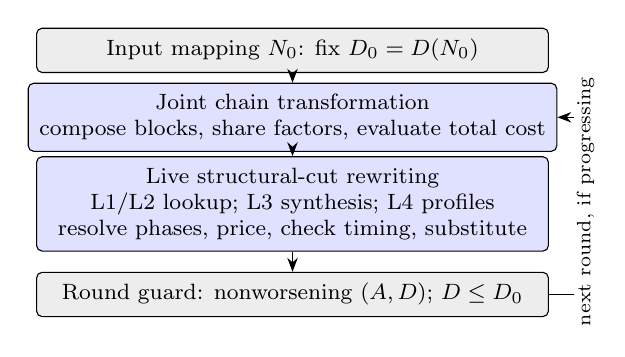
\begin{tikzpicture}[>=Stealth,font=\footnotesize,
 box/.style={draw,rounded corners=2pt,align=center,inner sep=4pt},
 arr/.style={->,line width=.45pt}]
 \node[box,fill=black!7,minimum width=6.5cm] (in) at (0,0) {Input mapping $N_0$: fix $D_0=D(N_0)$};
 \node[box,fill=blue!12,minimum width=6.5cm] (chain) at (0,-.85)
 {Joint chain transformation\\compose blocks, share factors, evaluate total cost};
 \node[box,fill=blue!12,minimum width=6.5cm] (cuts) at (0,-1.95)
 {Live structural-cut rewriting\\L1/L2 lookup; L3 synthesis; L4 profiles\\resolve phases, price, check timing, substitute};
 \node[box,fill=black!7,minimum width=6.5cm] (guard) at (0,-3.10)
 {Round guard: nonworsening $(A,D)$; $D\le D_0$};
 \draw[arr] (in)--(chain); \draw[arr] (chain)--(cuts); \draw[arr] (cuts)--(guard);
 \draw[arr] (guard.east)--++(.40,0)|- (chain.east);
 \node[rotate=90,font=\scriptsize,fill=white,inner sep=1pt] at (3.72,-1.92) {next round, if progressing};
\end{tikzpicture}}
\hfill
\subfloat[Two-step composition exposes a reusable product.]{%
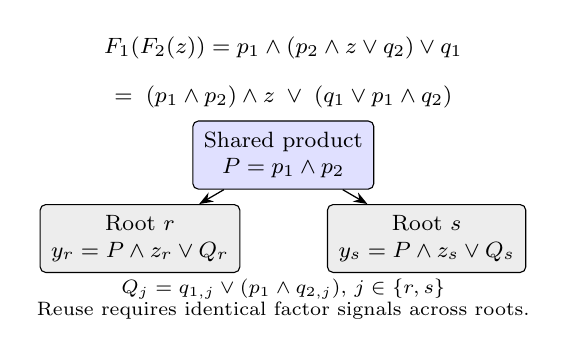
\begin{tikzpicture}[>=Stealth,font=\footnotesize,
 box/.style={draw,rounded corners=2pt,align=center,inner sep=4pt},
 arr/.style={->,line width=.45pt}]
 \node[align=center] at (0,0) {$F_1(F_2(z))=p_1\wedge(p_2\wedge z\vee q_2)\vee q_1$};
 \node[align=center] at (0,-.62) {$=\;(p_1\wedge p_2)\wedge z\;\vee\;(q_1\vee p_1\wedge q_2)$};
 \node[box,fill=blue!12] (prod) at (0,-1.36) {Shared product\\$P=p_1\wedge p_2$};
 \node[box,fill=black!7] (left) at (-1.82,-2.42) {Root $r$\\$y_r=P\wedge z_r\vee Q_r$};
 \node[box,fill=black!7] (right) at (1.82,-2.42) {Root $s$\\$y_s=P\wedge z_s\vee Q_s$};
 \draw[arr] (prod)--(left); \draw[arr] (prod)--(right);
 \node[align=center,font=\scriptsize] at (0,-3.19)
 {$Q_j=q_{1,j}\vee(p_1\wedge q_{2,j})$, $j\in\{r,s\}$\\Reuse requires identical factor signals across roots.};
\end{tikzpicture}}
\caption{Overview of ePMapping. (a) Joint chain transformation precedes local cut rewriting; both use the fixed initial delay bound and a final round check. (b) Two-step composition exposes a product $P$ reusable across roots with different residual functions $Q_j$. Acceptance accounts for all cells implementing the product, residual functions and outputs.}
\label{fig_layers}
\end{figure*}


\begin{algorithm}[t]
  \footnotesize
  \caption{A round of ePMapping.}\label{alg_epmapping}
  \KwIn{Mapped netlist $N$, initial delay bound $D_0$, library $\mathcal L$, maximum cut leaves $K$, retained-cut limit $B$, e-graph threshold $\theta$.}
  save a round backup of $N$ and its $(A,D)$ pair\;
  compose and share eligible AO21 chain blocks\;
  commit the transaction only if rebuilt area decreases and $D\le D_0$\;
  initialize a lazy cut manager for $N$ with bounds $K,B$\;
  \ForEach{live gate $x$ in reverse topological order}{
    $\mathit{best}\leftarrow\emptyset$\;
    \ForEach{nontrivial structural cut $\mathcal C=(x,L)$, $|L|\le K$}{
      compute $f_{\mathcal C}$ and its care mask\;
      $S\leftarrow\Call{SingleCell}{\mathcal C}\cup\Call{Database}{\mathcal C}\cup\Call{EligibleSynthesis}{\mathcal C}$\;
      $V\leftarrow$ proposals passing live phase, cost and timing checks\;
      \If{$V=\emptyset$ and $\mathcal C$ is the MFFC boundary cut and $A_{\rm rem}(x,L)\ge\theta$}{
        load or construct profiles; add feasible covers to $V$\;
      }
      update $\mathit{best}$ with the best proposal in $V$\;
    }
    \If{$\mathit{best}\ne\emptyset$ and it passes functional and cycle checks}{
      substitute $x$; update fanouts and timing; invalidate affected cuts\;
    }
  }
  rebuild $N$; restore the round backup if $D>D_0$ or $(A,D)$ worsens\;
\end{algorithm}

\subsection{Chain Blocks and Shared Factors}\label{sec:chain}
The chain stage exposes reuse that cannot be priced adequately by independent root substitutions. Consider a positive AO21 chain. An AO21 cell implements $y=(a\wedge b)\vee c$. Each chain step is $F_i(z)=(p_i\wedge z)\vee q_i$. A segment represents $(P,Q)$ with $F(z)=(P\wedge z)\vee Q$, and exact composition is
\begin{equation}
 (P,Q)\circ(p,q)=(P\wedge p,\;Q\vee(P\wedge q)).\label{eq:chain}
\end{equation}
Equation~\eqref{eq:chain} follows from Boolean distributivity and remains valid when coefficient signals are dependent. The optimization opportunity arises when identical products or segments can be reused by different roots.

Chains follow an AND input through single-fanout internal AO21 cells and stop at outputs or branching boundaries. Complemented fanin edges are excluded, although coefficient signals may be driven by explicit inverter cells. Traversal collects 6--64 steps per eligible segment, ordered from the root toward the boundary. Recursion splits off two-step blocks with balanced subdivision inside a block, terminating at $(0,z)$. This construction balances each block rather than the entire chain. Products use AND2--AND5 cells with arrival-aware physical pin assignment.

Product memo keys contain sorted unique factor signals; segment keys contain ordered coefficient pairs. Memoization spans roots, so identical factors and segments can be reused. All root proposals are constructed before substitution and treated as one transaction. Rebuilding counts every surviving cell, including the shared factors and residual functions. The transaction is retained only if total area strictly decreases and $D\le D_0$; otherwise the original netlist is restored. Subsequent cut rewriting may further simplify the resulting structures.

\subsection{Cover Representation and Feasibility}
All generators return a cell DAG with explicit polarities and physical pin assignments. Before phase resolution, a node $v$ with fanins $u_i$, pin delays $d_{v,i}$, input inversions $b_{v,i}$ and output inversion $o_v$ has arrival
\begin{equation}
 \tau_H(v)=\max_i\{\tau_H(u_i)+d_{v,i}+b_{v,i}d_{\rm inv}\}
                  +o_vd_{\rm inv}.\label{eq:delay}
\end{equation}
Here $\tau_H(\ell)=\tau(\ell)$ is the current arrival of leaf $\ell$. The binary flags $b_{v,i}$ and $o_v$ indicate input and output inversion, respectively, and $d_{\rm inv}$ is inverter delay. Pin delays are resolved by physical pin name, including permuted variants. Polarity flags describe inversions before emission; explicit inverter nodes are not charged a second time. Shared cover nodes are emitted once. Final area is the live-cell sum in \Cref{eq_area}. Area and timing are evaluated in the library model of \Cref{eq_area}.

Symbolic phase resolution precedes local selection and follows the same rules as materialization. If $u=\neg v$, a request for $\neg u$ uses $v$. An existing INV fanout can also supply $\neg u$, including a shared gate inside the root's fanin. It must have a live path to an output and must not depend on the replacement root. Explicit INV nodes and polarity flags use the same resolver; no cut is widened.

Let $M$ be the cut's removable cells, $J_H$ the existing cells retained by the resolved cover, and $V_H^{\rm new}$ its reachable new cells. The incremental implementation estimate is
\begin{equation}
 \widehat A_{\rm ctx}(H)=\sum_{v\in V_H^{\rm new}}a(v)+\sum_{v\in J_H\cap M}a(v).\label{eq:context_area}
\end{equation}
Existing shared cells outside $M$ add no area; retaining a removable gate is charged. Cancelled and unreachable new nodes are excluded. Timing is propagated on the resolved DAG using actual arrivals at reused signals. Rebuilt netlist measurements guard the combined result. The winning cover is checked on care minterms; final CEC validates rewrite interactions.

Care computation projects a bounded reconvergence simulation onto cut leaves. Free inputs over-approximate surrounding logic, so only conservatively unreachable minterms become DCs. Cuts outside the window remain fully specified. SAT refinement is disabled. L1, L2 and SOP factoring can exploit partial functions; cofactor candidates and L4 use the fully specified function.

\subsection{Four Complementary Cover Generators}
\begin{table}[t]
  \centering\footnotesize
  \caption{Cover generators and their practical limits. L1--L3 compete on eligible cuts; L4 is a fallback after acceptance filtering.}\label{tab:layers}
  \tabcolsep=3pt
  \begin{tabular}{@{}l >{\raggedright\arraybackslash}p{3.05cm} >{\raggedright\arraybackslash}p{3.05cm}@{}}
    \toprule
    Generator & Mechanism & Limit \\
    \midrule
    L1 single cell & indexed function, input phases and permutations & one cell; bounded DC completions \\
    L2 database & pre-mapped four-input cell DAGs & stored functions and entry limits \\
    L3 synthesis & SOP/DSD, Shannon and Davio decompositions & bounded support and heuristic mapping \\
    L4 e-graph & AIG rewrites and library cover rules & rewrite reachability, saturation budget and heuristic extraction \\
    \bottomrule
  \end{tabular}
\end{table}

\paragraph{L1: indexed single-cell matching}
The library index includes input permutations and polarities and probes both output phases. Partial-function matching enumerates completions under free-minterm and entry caps.

\paragraph{L2: mapped sub-network lookup}
ABC's \texttt{super} builds the database offline. A separate library supplies lookup and internal cut mapping without changing initial \texttt{emap}; noDB removes both uses.

\paragraph{L3: structural synthesis}
Sum-of-products (SOP) factoring and disjoint-support decomposition (DSD) build AIGs and map them to the library. A compact factorization is only one choice. For $f=f_{\mathcal C}$ and a retained pivot $\ell\in L$, let $f_b=f|_{\ell=b}$. We independently construct and map
\begin{align}
 f&=(\ell\wedge f_1)\vee(\neg\ell\wedge f_0),\nonumber\\
 f&=f_0\oplus[\ell\wedge(f_0\oplus f_1)]\nonumber\\
  &=f_1\oplus[\neg\ell\wedge(f_0\oplus f_1)].\label{eq:decomp}
\end{align}
The first is Shannon decomposition; the latter two are positive/negative Davio forms. Cofactors and Boolean differences are SOP-factored before mapping. These candidates implement the fully specified cut function and are checked over its entire truth table. They compete with the other sources under the same timing bound.

We retain two pivots per decomposition family. Let $s(g)$ be the number of variables in the support of $g$, and let $\Delta_\ell=f_0\oplus f_1$. Shannon ranks pivots by $s(f_0)+s(f_1)$; positive and negative Davio use $s(f_0)+s(\Delta_\ell)$ and $s(f_1)+s(\Delta_\ell)$, respectively. Ties follow leaf order; retained pivots are processed in their original order. This structural budget reduces candidate construction but can omit useful covers. Timing feasibility is checked after mapping, not inferred from support size.

For example, $d\wedge(\neg c\vee a)\wedge(c\vee b)$ equals $(d\wedge c\wedge a)\vee(d\wedge\neg c\wedge b)$. The latter can use an AO33 with $d$ connected to two pins. The six-pin cell then implements a four-variable function, a binding not enumerated by the direct single-cell matcher. Decomposition changes the available library covers rather than just enlarging an extraction front.

\subsection{Equality Saturation for Cover Generation}\label{sec:egg}
\paragraph{Language and rules}
Each input cell is expanded through its genlib expression into an AIG. Gate symbols and AIG nodes coexist; truth-table analysis checks merged e-classes. Static rules cover double-negation elimination/insertion, AND commutativity and reassociation, complements, idempotence and constants. Library rules replace matching AIG expressions with cells. Cell-to-AIG expansion is omitted because the seed is already expanded. The budget is two iterations and 500 e-nodes; this local search does not systematically enumerate the decompositions in \Cref{eq:decomp}.

\paragraph{Extraction}
Extraction is independent of current leaf arrivals. A worklist retains cell DAGs with alternative pins and child realizations. A narrow pass first keeps one area-oriented realization per e-class, using at most one quarter of the combination allowance and half the visit allowance. The wider pass starts from these realizations and receives all unused work. Both passes together obey the original limits; the narrow pass reserves inexpensive coverage before wider Cartesian enumeration. Structural interning shares identical nodes. Child dependencies containing the current e-class are excluded to bound recursive unrolling. Raw AIG nodes require AND and inverter cells.

For a cover $H$, let $U_H\subseteq L$ be its used inputs and $p_i(H)$ the longest input-to-root delay, including polarity costs. Its current arrival is
\begin{equation}\label{eq:profile}
T(H;\boldsymbol{\tau})=\max_{i\in U_H}\{\tau(\ell_i)+p_i(H)\}.
\end{equation}
Constant covers have zero arrival in this model. The stored profile is $(\widehat A(H),p_0(H),\ldots,p_{|L|-1}(H))$. Unused coordinates are ignored in timing and treated as $-\infty$ for dominance. Root pruning compares area and every delay coordinate, avoiding scalar zero-arrival pruning. Distinct intermediate structures can survive standalone dominance because parents may share their nodes. Caps make this an incomplete candidate pool; intrinsic profiles also omit external reuse.

Persistent keys include the expanded AIG seed, variable order, library, extraction version, limits and retention settings, excluding arrivals and required times. Hits load DAGs and vectors; misses saturate and extract. Pin variants are enumerated only for cells in the bounded DAG; invalid records are rebuilt. Empty pools retry single-realization extraction. With contextual pricing, intrinsic rounded-arrival filtering is bypassed: phase resolution may improve timing. Selection uses unrounded live costs; bounded intrinsic pruning can still omit useful context-dependent covers.

\subsection{Acceptance and Iteration}\label{sec:accept}
Backward required times implement \Cref{eq:objective}. For an output, $R(o)=D_0$; for an internal signal,
\begin{equation}
 R(u)=\min_{(u,v,i)}\{R(v)-d_{v,i}-b_{v,i}d_{\rm inv}\},\label{eq:required}
\end{equation}
with output inversions deducted at the boundary. The minimum ranges over live fanout pins. A cover is timing-feasible when its recomputed root arrival does not exceed $R(x)$ within tolerance. Required-time caches are invalidated after substitution, so a noncritical rewrite may consume current slack without relaxing $D_0$.

Across cuts, candidates rank by $\widehat A_{\rm ctx}(H)-A_{\rm rem}(x,L)$, then root arrival and structural level. Here $A_{\rm rem}=\sum_{v\in M}a(v)$; shared existing logic is not assumed removable. Functional and cycle checks precede substitution. A rebuilt round must respect $D_0$ and not worsen the quantized $(A,D)$ pair, or it is restored.

The bound spans all rounds. A faster but larger result is rejected; delay and then level break area ties. Area and delay keys are quantized to $10^{-4}$ and $10^{-3}$, respectively. Roots without admissible covers are skipped. The evaluated method uses neither whole-window synthesis nor unmap/remap exploration. Reconvergence-window simulation is used only to compute cut care sets.

Rounds stop on no substitution, no objective progress, or the round cap.

\subsection{Reusing Construction Work}\label{sec:buildreuse}
Native synthesis caches support, ordered truth tables, mode and objective; SOP keys include DCs and cofactor keys the pivot. A second cache reuses mapped DAGs and full-function proofs across cofactor requests with identical pre-mapping AIG states. Keys preserve PI/PO order, every node slot, edge phases, reference counts and traversal state. Library and mapper settings are fixed. No contextual price is cached across network changes. Request caches retain entries across rounds; transient mapped networks share an owned immutable library.

For an area-first cut, sum root-reachable non-inverter cell areas, counting shared nodes once. This lower bound excludes inverter costs and retained removable gates; other cells are emitted anew. Live pricing is omitted only when the bound exceeds a feasible incumbent area by more than $10^{-3}$, or the original cone area if no incumbent exists. Area ties remain eligible. Fresh SOP/DSD and cofactor covers are priced once per unchanged cut.

Inverse-phase queries cache both a reusable live inverter and a negative result. Entries are valid only for one root, network revision and node-slot count; substitution, rebuilding or candidate-node insertion invalidates them. An inverter at a strictly lower structural level cannot depend on the root; remaining cases retain the dependency traversal. Cut simulation decodes gate functions and fanins once, reuses scratch storage, and supplies the cached truth table to repeated requests. These mechanisms reuse computation; the pivot budget separately restricts search.

Every statistical deferral is rechecked in its original position before root commitment. Only strict area dominance skips live pricing among the generated covers.

Periodically after substitutions and at round ends, a rebuilt copy is saved if it meets the original area/delay bounds and improves the best quantized objective. The initial mapping is saved first. A deadline leaves the search incomplete; independent CEC and serialized-netlist audits admit the saved output. Snapshot construction and writing consume the post-mapping budget.

\begin{figure*}[t]
\centering
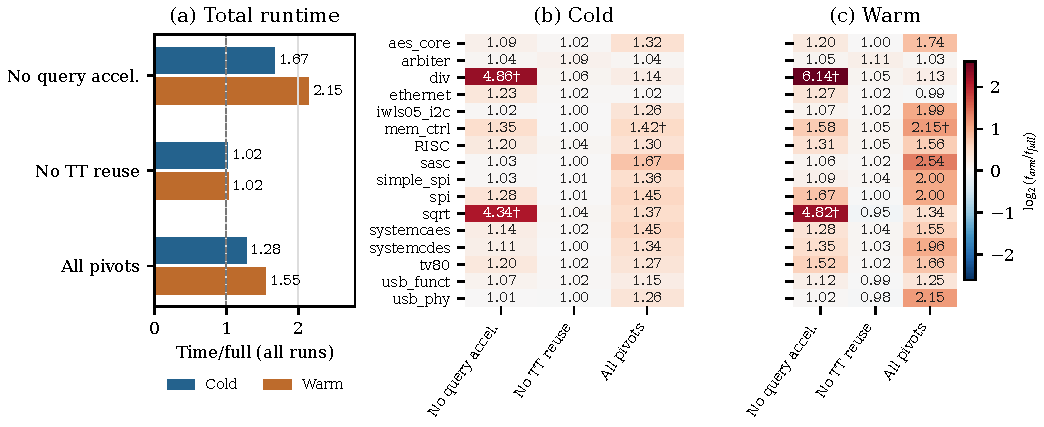
\includegraphics[width=\textwidth]{results/build_ablation.pdf}
\caption{Query, truth-table and pivot-control runtime relative to full, cold/warm: aggregate optimizer-time ratios and per-design ratios. Colors encode the logarithm of each ratio. $\dagger$ marks at least one TO; equal elapsed budgets do not imply equal completed work. Selected-output area effects and timeout counts appear in \Cref{tab:ablation}.}\label{fig:ablation}
\end{figure*}

\begin{figure}[t]
\centering
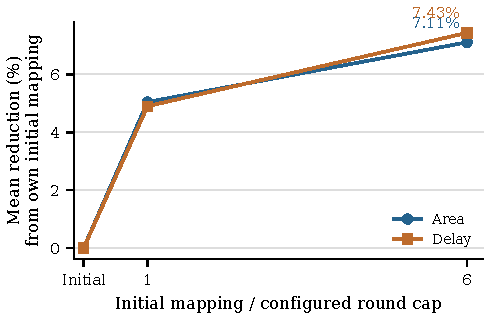
\includegraphics[width=.90\linewidth]{results/round_progress.pdf}
\caption{Selected-output reductions from $N_e$ at caps 1 and 6. Cold/warm curves separate when different; intermediate caps were not measured.}\label{fig:rounds}
\end{figure}
\section{Experimental Results}

\MfsComparisonTable
\MainResultTable
\subsection{Setup}\label{sec:setup}
We evaluate sixteen designs with the ASAP7 genlib~\cite{asap7}, reporting area in $\mu m^2$ and worst-output delay in ps. We use C++/mockturtle~\cite{EPFLLibraries}, Rust/\textit{egg}~\cite{willsey2021egg}, and ABC~\cite{ABCTool}.

All experiments fix the initial delay bound across rounds (\Cref{eq:objective}), with whole-window synthesis and unmap/remap exploration disabled.

For \texttt{mfs3}, both tools use the same 40-entry subset with at most six inputs per cell, and byte-identical area-oriented \texttt{emap} inputs. The evaluated \texttt{mfs3} implementation restricts cell truth tables and node simulation to six inputs. Preprocessing experiments and ablations use all 47 entries for initial mapping and optimization.

The direct input $N_i$ maps the raw AIG without ABC optimization. For $N_e$, the flow repeats \texttt{fraig; resyn2rs; fraig; compress2rs} until the AND count stops decreasing, with a 20-iteration cap, then applies area-oriented \texttt{emap}. Let $A_e=A(N_e)$ and $D_e=D(N_e)$.

Cuts use $K=6$, $B=12$ and $\theta=0$. Care uses an eight-input reconvergence window and 60\,s cumulative budget, then full care; SAT refinement is off. The three-level database has area cap $0.50$. SOP/DSD starts at four leaves; Shannon/Davio at three, with two ranked pivots per family. Each native structure cache holds 262144 entries. Independent polarity factoring and exact AIG synthesis are off. L4 allows two iterations, 500 e-nodes, eight realizations per class, 20000 combinations and 4000 visits. Chain blocks have two steps and minimum length six. Round caps allow early stopping.

Experiments run on two Xeon Gold 6226R sockets (32 cores), Ubuntu 22.04.5, GCC 11.2.0, Rust 1.99.0 and ABC 1.01. A shared host runs up to twelve single-worker ePMapping optimizations and six independent ABC jobs. Both tools have a 1000\,s post-mapping limit. For ePMapping this includes optimizer preparation, all rounds and final rebuild, excluding preprocessing, mapping and CEC. An outer 3600\,s guard covers setup and validation.

Each configuration/design runs cold with an empty private pool, then warm with the same pool and limits. Native caches restart; OS caches are not cleared. Both groups share the verified ABC batch. Times are $t_c/t_w$. Externally interrupted attempts are archived, excluded from timing totals, and retried with their prescribed cache state.

Completed and selected deadline outputs undergo CEC and independent serialized-PPA audits. A TO remains incomplete: the best legal checkpoint is selected, or the initial mapping. Snapshot costs count toward 1000\,s; post-run validation does not. Interrupted ABC runs retain the initial mapping. \FullCompletionSentence{} Across all parts, cold/warm have \ColdCompleted{}/\WarmCompleted{} completions and \ColdMethodTimeouts{}/\WarmMethodTimeouts{} timeouts; \ColdCheckpointSelections{}/\WarmCheckpointSelections{} timeouts select improved checkpoints. Differing costs are stacked or separated by a slash, cold first. Define $\delta A_j=100(A_j/A_{0,j}-1)$ and $\delta D_j=100(D_j/D_{0,j}-1)$. Means include initial selections; ablations sum $\Delta A=\sum_j(A_{\rm arm,j}-A_{\rm full,j})$.

\subsection{Area Recovery after AIG Preprocessing}\label{sec:aspdac}

Both preprocessing-experiment caps start from $N_e$ (\Cref{tab:main}). At one round, mean area changes are \OwnOneArea\%; mean delay changes are \OwnOneDelay\% (cold/warm). At cap 6, these are \OwnArea\% area and \OwnDelay\% delay, with \ColdMainCompleted{}/\WarmMainCompleted{} completed runs. Area decreases on \OwnAreaWins{} of sixteen; all selected outputs meet the initial bounds. The caps are measured independently.

For \texttt{arbiter}, area changes from $557.72$ to $\ArbiterArea\,\mu m^2$ and delay from $999.87$ to $\ArbiterDelay$\,ps. The other fifteen average \mbox{\OwnOtherArea\%} area and \mbox{\OwnOtherDelay\%} delay changes.



ASPDAC'25 costs are reconstructed from its reported starts and rounded changes~\cite{aspdac25}; its implementation is unavailable. Our final area is smaller on \MainWins{} designs, with mean area and delay differences of \mbox{\MainAreaAll\%} and \mbox{\MainDelayAll\%}. These approximate comparisons use different starts and cannot isolate post-mapping gains; our delay bound refers to our input.

\subsection{Common-Input Comparison with ABC}\label{sec:mfs3}
Both tools receive the same direct mapping (\Cref{tab:mfs3}); ours uses one round. ABC's \texttt{mfs3 -a} does not enforce our initial-delay bound, so we distinguish raw and externally guarded outputs.

ABC completes \ABCCompleted{} designs and times out on \ABCTimeouts{}. On the ABC-completed subset, its mean area/delay changes are \mbox{\ABCArea\%}/\mbox{\ABCDelay\%}, versus \mbox{\PairedOwnArea\%}/\mbox{\PairedOwnDelay\%} for our verified selections. ePMapping completes \ColdMfsCompleted{}/\WarmMfsCompleted{} designs cold/warm. Its all-sixteen selected-output means are \mbox{\MfsOwnArea\%}/\mbox{\MfsOwnDelay\%}, within the initial delay bounds.

Of the completed ABC outputs, \ABCViolations{} violate the delay bound and \ABCFeasible{} satisfy both bounds. An external guard retains only feasible outputs, otherwise selecting the initial mapping; its paired means are \mbox{\ABCGuardArea\%} area and \mbox{\ABCGuardDelay\%} delay. This guard leaves ABC unchanged.

Ratios in \Cref{tab:mfs3} use each tool's native initial costs: ABC import may normalize output buffers. Times exclude CEC; ABC includes import and writing, ours optimizer preparation through rebuild.

\subsection{Operator Ablations and Efficiency}\label{sec:oracles}
\AblationResultTable


All nineteen arms use identical $N_e$ starts and bounds (\Cref{tab:ablation}); L1 stays enabled. noSYN removes L3, noEGG removes L4, noDB removes lookup and database-derived mapper entries, and noCARE supplies full care. noCHAIN skips composition; noSHARE clears chain memo tables between roots. noNARROW removes narrow initialization; noPHASE disables physical phase reuse.

noSHANNON retains Davio only; noDAVIO retains Shannon only. noREUSE removes forward INV lookup but keeps backward cancellation; noPRICE removes contextual pricing while preserving physical reuse. noQUERY restores uncached inverse queries and dependency traversal. noTRUTH disables decoded simulation and dynamic-table reuse; the common scalar cut memo remains. allPIVOTS removes the pivot cap. cache64K uses 65536 native entries, noAIGREUSE disables pre-mapping AIG reuse, and noLIBSHARE copies libraries.

The noQUERY and noTRUTH time/full ratios are \QueryColdRatio{}/\QueryWarmRatio{} and \TruthColdRatio{}/\TruthWarmRatio{}. allPIVOTS has ratio \PivotColdRatio{}/\PivotWarmRatio{} and summed area differences \PivotAreaCold{}/\PivotAreaWarm{}\,$\mu m^2$. noTRUTH leaves every final area and delay unchanged. Unrestricted pivots recover more area overall but time out on \texttt{mem\_ctrl} cold and warm (\Cref{fig:ablation}).

Removing Shannon and Davio gives summed area differences of \DeltaShannon{} and \DeltaDavio\,$\mu m^2$; removing forward reuse and live pricing gives \DeltaReuse{} and \DeltaPrice\,$\mu m^2$. \UsbAblationExample{} Independent runs can follow different trajectories under care budgets and deadlines. \DeadlineExample{}

noDB improves \DBBetterCount{} designs but changes both lookup and inner mapping. Ablation effects are not additive.

Removing L4 worsens area on \EggWorseCount{} designs; its cold/warm time ratios are \ColdNoEggRatio{}/\WarmNoEggRatio{}. L4 takes \TimeEggShare\%/\WarmTimeEggShare\% of recorded phase time in \ColdPhaseRuns{}/\WarmPhaseRuns{} completed full runs (CEC and other phases excluded). Pool hits avoid saturation and extraction; native caches restart per process. TO ratios compare elapsed budgets, not equal completed work. \CacheDeadlineExample{} Shared-host scheduling affects elapsed time.


\section{Conclusion}
ePMapping combines shared AO21 blocks, cut decompositions, reusable arrival-independent profiles and live phase pricing under the initial delay bound. Query, truth-table and construction reuse avoid repeated work; support-ranked pivots limit candidate generation. The experiments measure area recovery and runtime separately. Finite candidate pools and pivot budgets can still omit useful implementations.


\clearpage
\IEEEtriggeratref{9}
\bibliographystyle{IEEEtran}
\bibliography{ref/Top-sim,ref/all}

\end{document}
